% =============================================================================
%  02-prancha-ilustrativa-A3.tex — prancha A3 (paisagem) com moldura, zonas e
%  legenda no padrão das folhas de desenho técnico (ABNT NBR 10068: margem
%  esquerda de 25 mm, demais de 7 mm; legenda de 178 mm no canto inferior
%  direito). Coordenadas em milímetros a partir do canto inferior esquerdo.
%  Pré-requisito: figuras/figs-prancha.pdf e figuras/tempos-a3.pdf.
%  Compilar com pdflatex duas vezes (remember picture).
% =============================================================================
\documentclass{article}
\usepackage[a3paper, landscape, margin=0mm]{geometry}
\usepackage{projeto-sabado}
\usepackage[scaled=0.95]{helvet}
\renewcommand{\familydefault}{\sfdefault}
\pagestyle{empty}
\hypersetup{pdftitle={Prancha ilustrativa A3 — projeto\_sabado (NE555 + CD4017B)}}

% painel: \painel{x0}{y0}{x1}{y1}{título}
\newcommand{\painel}[5]{%
  \draw[charcoal, line width=0.3mm] (#1,#2) rectangle (#3,#4);
  \fill[petroleo] (#1,#4-5.2) rectangle (#3,#4);
  \node[anchor=west, text=white, font=\footnotesize\bfseries, inner sep=0] at (#1+2,#4-2.6) {#5};}
% campo da legenda: \campo{x0}{y0}{x1}{y1}{rótulo}{valor}
\newcommand{\campo}[6]{%
  \draw[charcoal, line width=0.2mm] (#1,#2) rectangle (#3,#4);
  \node[anchor=base west, font=\tiny, text=charcoal!80, inner sep=0] at (#1+1.2,#4-3.0) {#5};
  \node[anchor=base west, font=\footnotesize\bfseries, inner sep=0] at (#1+1.2,#2+2.6) {#6};}

\begin{document}
\noindent\begin{tikzpicture}[remember picture, overlay, x=1mm, y=1mm]
\begin{scope}[shift={(current page.south west)}]

% ------------------------------------------------------------------ moldura e zonas
\draw[charcoal, line width=0.7mm] (25,7) rectangle (413,290);
\draw[charcoal, line width=0.25mm] (30,12) rectangle (408,285);
\foreach \i in {1,...,8}{
  \pgfmathsetmacro{\xc}{30+(\i-0.5)*378/8}
  \node[font=\scriptsize, text=charcoal] at (\xc,287.5) {\i};
  \node[font=\scriptsize, text=charcoal] at (\xc,9.5) {\i};}
\foreach \i in {1,...,7}{
  \pgfmathsetmacro{\xd}{30+\i*378/8}
  \draw[charcoal, line width=0.25mm] (\xd,285) -- (\xd,290) (\xd,7) -- (\xd,12);}
\foreach \l [count=\i] in {A,B,C,D,E,F}{
  \pgfmathsetmacro{\yc}{285-(\i-0.5)*273/6}
  \node[font=\scriptsize, text=charcoal] at (27.5,\yc) {\l};
  \node[font=\scriptsize, text=charcoal] at (410.5,\yc) {\l};}
\foreach \i in {1,...,5}{
  \pgfmathsetmacro{\yd}{285-\i*273/6}
  \draw[charcoal, line width=0.25mm] (25,\yd) -- (30,\yd) (408,\yd) -- (413,\yd);}
% marcas de centro
\draw[charcoal, line width=0.5mm] (219,285) -- (219,292) (219,12) -- (219,5)
  (30,148.5) -- (23,148.5) (408,148.5) -- (415,148.5);

% ------------------------------------------------------------------ faixa de título
\node[anchor=west, font=\Large\bfseries, text=petroleo, inner sep=0] at (32,280.6)
  {SEQUENCIAL DE 6 LEDs COM NE555 E CD4017B};
\node[anchor=west, font=\small, text=charcoal, inner sep=0] at (168,280.6)
  {prancha ilustrativa de especificações e ligações · esquemático \texttt{projeto\_sabado} (Rev.\,01)};
\draw[dourado, line width=0.6mm] (30,276.4) -- (408,276.4);

% ------------------------------------------------------------------ P1 esquemático
\painel{30}{166}{282}{274}{1 · DIAGRAMA ESQUEMÁTICO — redesenho com a mesma lista de ligações do original}
\node[anchor=north, inner sep=0] at (156,267.6)
  {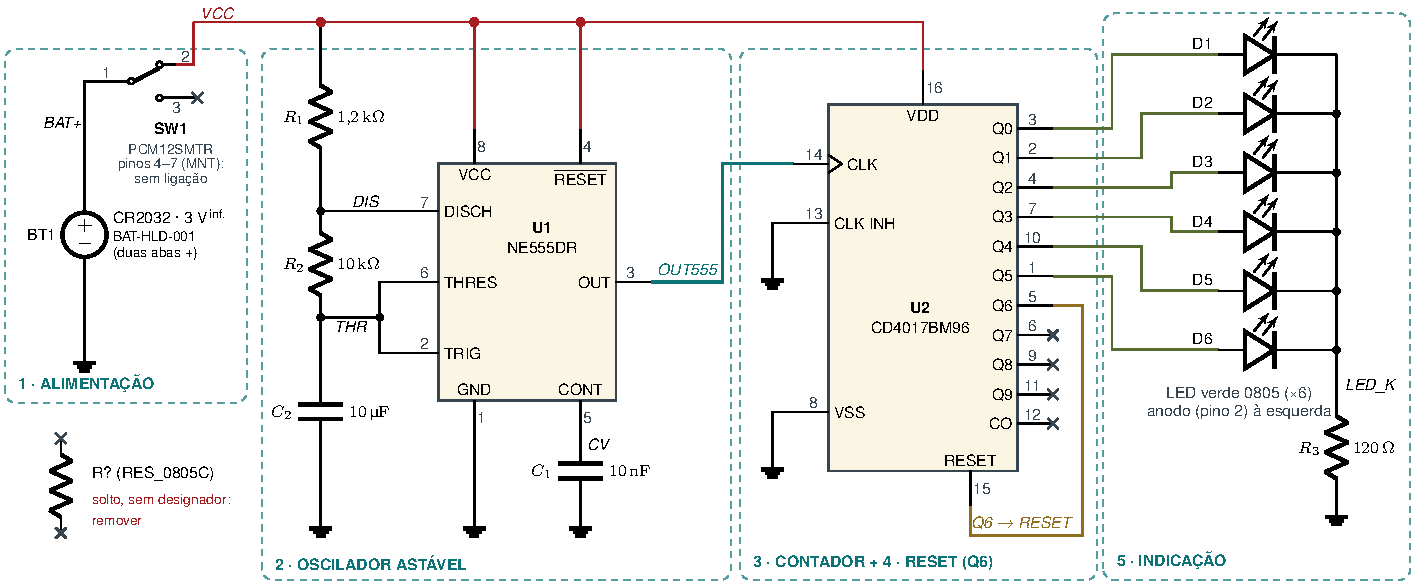
\includegraphics[page=1]{figuras/figs-prancha.pdf}};

% ------------------------------------------------------------------ P2 BOM + notas
\painel{285}{166}{408}{274}{2 · LISTA DE MATERIAIS E NOTAS TÉCNICAS}
\node[anchor=north west, inner sep=0] at (287,267)
{\fontsize{6.8}{8.1}\selectfont
\begin{tabular}{@{}l l l >{\raggedright\arraybackslash}p{37mm} >{\raggedright\arraybackslash}p{25mm}@{}}
\toprule
\textbf{Ref.} & \textbf{Valor} & \textbf{Encaps.} & \textbf{Fabricante / código} & \textbf{Função} \\
\midrule
BT1 & CR2032 3 V\textsuperscript{*} & SMT & Linx/TE BAT-HLD-001 & bateria (fonte) \\
SW1 & SPDT & SMT & C\&K PCM12SMTR & liga/desliga \\
U1 & 555 bipolar & SOIC-8 & TI NE555DR & oscilador astável \\
U2 & contador & SOIC-16 & TI CD4017BM96 & sequenciador \\
R1 & 1,2 k$\Omega$ & 0805 & Yageo RC0805FR-071K2L\textsuperscript{*} & temporização ($R_A$) \\
R2 & 10 k$\Omega$ & 0805 & Yageo RC0805FR-0710KL\textsuperscript{*} & temporização ($R_B$) \\
R3 & 120 $\Omega$ & 0805 & Yageo RC0805FR-07120RL\textsuperscript{*} & resistor comum dos LEDs \\
C1 & 10 nF X7R\textsuperscript{*} & 0805 & Murata GRM216R71H103KA01\textsuperscript{*} & desacopla o CONT \\
C2 & 10 µF X5R\textsuperscript{*} & 0805 & Murata GRM21BR61A106KE19\textsuperscript{*} & capacitor de tempo \\
D1–D6 & LED verde & 0805 & Kingbright APT2012SGC\textsuperscript{*} & indicação (×6) \\
\midrule
R? & — & 0805 & RES\_0805C (solto) & \textcolor{redeVcc}{remover} \\
\bottomrule
\multicolumn{5}{@{}l}{\textsuperscript{*}\,inferido: o print não mostra a bateria, o dielétrico nem o fabricante dos passivos e LEDs.}
\end{tabular}};
\node[anchor=north west, inner sep=0, text width=119mm, align=left] at (287,218.5)
{\fontsize{6.8}{8.2}\selectfont\raggedright
\textbf{\color{petroleo}NOTAS TÉCNICAS (revisão por datasheet)}\\[0.6mm]
\textbf{N1.} NE555 é especificado de 4,5 a 16 V; com CR2032 (3 V, corte em 2 V) fica \textcolor{redeVcc}{fora da faixa}, e seu nível alto ($\approx V_{CC}-1{,}3$ V $\approx$ 1,7 V) nem chega ao $V_{IH}$ do 4017. Trocar por LMC555 ($\geq$1,5 V) ou TLC555C ($\geq$2 V). O CD4017B ($\geq$3 V) também fica abaixo do mínimo sob carga: o CD74HC4017 (2 a 6 V) tem a mesma pinagem.\\[0.5mm]
\textbf{N2.} Não há desacoplamento: incluir 100 nF X7R junto a U1-8 e U2-16 e 10 a 47 µF junto à bateria (evita clock falso no CD4017B).\\[0.5mm]
\textbf{N3.} O resistor R? está solto e sem designador: apagar e rodar Annotate + ERC antes do layout.\\[0.5mm]
\textbf{N4.} C2 cerâmico de 10 µF perde capacitância com tensão DC: a frequência sobe. Mesma $f$ com R1 = 10 k$\Omega$, R2 = 100 k$\Omega$, C2 = 1 µF X7R ($f \approx 6{,}87$ Hz).\\[0.5mm]
\textbf{N5.} Usar LED verde de baixa Vf (GaP, 568 nm, 2,2 V típ. a 20 mA). O InGaN (525 nm, 3,3 V típ.) pode não acender a 3 V.\\[0.5mm]
\textbf{N6.} Q6 $\to$ RESET direto: o pulso se encerra sozinho ($\approx$265 ns típ. a 5 V), perto da largura mínima de 260 ns. Funciona; a versão robusta usa flip-flop S-R (datasheet, Fig. 18).\\[0.5mm]
\textbf{N7.} BT1: o negativo é uma ilha de cobre de Ø 18 mm na própria placa, exposta e ligada ao GND.};

% ------------------------------------------------------------------ P3 pinagem
\painel{30}{79}{282}{163}{3 · PINAGEM DOS CIs — vista superior, terminal colorido conforme a rede}
\node[anchor=north west, inner sep=0] at (31,156.5)
  {\includegraphics[page=2, scale=0.92]{figuras/figs-prancha.pdf}};
\node[anchor=north east, inner sep=0] at (281,156.5)
  {\includegraphics[page=3, scale=0.92]{figuras/figs-prancha.pdf}};
\node[anchor=north west, inner sep=0, text width=118mm, align=left] at (34,108)
{\fontsize{6.8}{8.2}\selectfont
\textbf{\color{petroleo}ENCAPSULAMENTOS}\\[0.5mm]
SOIC-8 (D) e SOIC-16 (D/M): corpo de 3,9 mm de largura, passo de 1,27 mm; 4,9 mm
(8 pinos) e 9,9 mm (16 pinos) de comprimento. Desenho ampliado cerca de 6,9:1.\\
Ponto no canto = pino 1. Passivos e LEDs 0805: 2,0 $\times$ 1,25 mm.\\[0.8mm]
\textbf{\color{petroleo}ORDEM FÍSICA DAS SAÍDAS DO CD4017B}\\[0.5mm]
Q0 = 3, Q1 = 2, Q2 = 4, Q3 = 7, Q4 = 10, Q5 = 1, Q6 = 5, Q7 = 6, Q8 = 9, Q9 = 11.
As saídas não seguem a ordem dos pinos: erro clássico de roteamento.};

% ------------------------------------------------------------------ P4 diagrama de tempos
\painel{285}{79}{408}{163}{4 · DIAGRAMA DE TEMPOS (regime permanente)}
\node[anchor=north, inner sep=0] at (346.5,156)
  {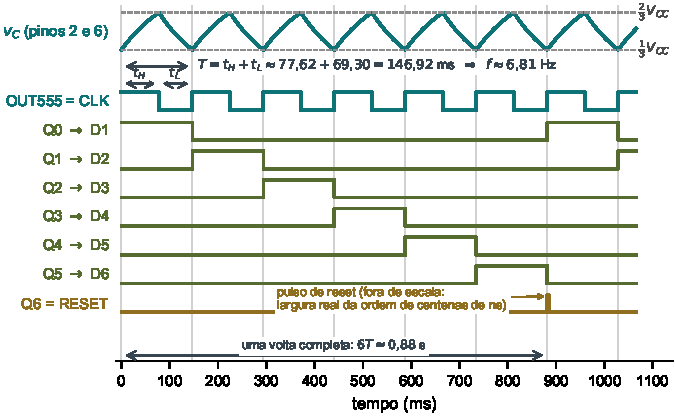
\includegraphics[width=119mm]{figuras/tempos-a3.pdf}};

% ------------------------------------------------------------------ P5 diagrama de blocos
\painel{30}{12}{175}{76}{5 · DIAGRAMA DE BLOCOS FUNCIONAL}
\node[anchor=north, inner sep=0] at (102.5,69.5)
  {\includegraphics[page=5, width=139mm]{figuras/figs-prancha.pdf}};

% ------------------------------------------------------------------ P6 dados de projeto
\painel{178}{12}{227}{76}{6 · DADOS DE PROJETO}
\node[anchor=north west, inner sep=0, text width=46mm, align=left] at (179.5,69)
{\fontsize{6.8}{8.6}\selectfont
VCC $\approx$ 3 V (CR2032, 2,0 a 3,2 V)\\
$t_H = 0{,}693\,(R_1{+}R_2)\,C_2 \approx 77{,}62$ ms\\
$t_L = 0{,}693\,R_2\,C_2 \approx 69{,}30$ ms\\
$T = t_H + t_L \approx 146{,}92$ ms\\
$f = 1/T \approx 6{,}81$ Hz\\
$D = (R_1{+}R_2)/(R_1{+}2R_2) \approx 52{,}83\,\%$\\
1 LED por período $T$\\
volta de 6 LEDs: $6T \approx 0{,}88$ s\\
$I_{\text{LED}} \approx 0{,}5$ a 1,5 mA (saída CMOS)\\
consumo como está: 3,68 a 5,73 mA\\
consumo revisado: 0,79 a 1,84 mA\\
{\color{charcoal!80}(revisado = LMC555 + RC da N4)}};

% ------------------------------------------------------------------ convenções
\draw[charcoal, line width=0.3mm] (230,65) rectangle (408,76);
\node[anchor=north west, font=\fontsize{6.5}{7.5}\selectfont\bfseries, text=petroleo, inner sep=0] at (231.5,74.8) {CONVENÇÕES DE REDE};
\node[anchor=north west, inner sep=0] at (231.5,71.4)
  {\includegraphics[page=4, width=150mm]{figuras/figs-prancha.pdf}};
\node[anchor=north east, font=\fontsize{6}{7}\selectfont, text=charcoal, inner sep=0] at (406.5,74.8)
  {× = sem conexão (NC) · ponto = junção};

% ------------------------------------------------------------------ legenda (carimbo)
\fill[white] (230,12) rectangle (408,62);
\draw[charcoal, line width=0.5mm] (230,12) rectangle (408,62);
\fill[petroleo] (230,53) rectangle (408,62);
\node[anchor=west, text=white, font=\footnotesize\bfseries, inner sep=0] at (233,57.5)
  {DEMONSTRAÇÃO · PROJETO TÉCNICO ASSISTIDO POR LLM};
\node[anchor=east, text=white, font=\scriptsize, inner sep=0] at (405,57.5) {Prancha 02 do conjunto 01–03};
\draw[charcoal, line width=0.2mm] (230,37) rectangle (408,53);
\node[anchor=north west, font=\tiny, text=charcoal!80, inner sep=0] at (231.2,52) {TÍTULO};
\node[anchor=west, font=\normalsize\bfseries, inner sep=0] at (231.2,46.2) {Sequencial de 6 LEDs com NE555 e CD4017B};
\node[anchor=west, font=\scriptsize, inner sep=0] at (231.2,40.6) {Prancha ilustrativa de especificações, pinagem e ligações};
\draw[charcoal, line width=0.2mm] (230,25) rectangle (408,37);
\node[anchor=north west, font=\tiny, text=charcoal!80, inner sep=0] at (231.2,36) {PROJETO DE ORIGEM};
\node[anchor=west, font=\scriptsize, inner sep=0] at (231.2,29.6)
  {\texttt{projeto\_sabado} · JuliaLabs (YouTube, 19/11/2026) · Altium Designer · Sheet1.SchDoc, Rev.\,01};
\campo{230}{12}{259.7}{25}{FORMATO}{A3}
\campo{259.7}{12}{289.4}{25}{ESCALA}{sem escala}
\campo{289.4}{12}{319.1}{25}{UNIDADES}{SI · vírgula}
\campo{319.1}{12}{348.8}{25}{DATA}{21/11/2026}
\campo{348.8}{12}{378.5}{25}{REVISÃO}{1.0 (orig. Rev. 01)}
\campo{378.5}{12}{408}{25}{FOLHA}{1/1}

\end{scope}
\end{tikzpicture}
\end{document}
